\chapter{Implementazione della piattaforma}
\fancyhead[RO]{\bfseries Implementazione della piattaforma}

La piattaforma deve riuscire a conciliare i bisogni di due attori molto diversi, il publisher e il subscriber.
Il primo, che possiamo identificare nel possessore di un sensore, vuole pubblicare i suoi dati sulla piattaforma in sicurezza e nella maniera più semplice. I subscribers invece, sono tutte le aziende che creano applicazioni utilizzando quei dati, quest'ultimi hanno bisogno di massima integrazione per rendere facile e veloce lo sviluppo e l'adozione del software.
\begin{figure}
\begin{center}
 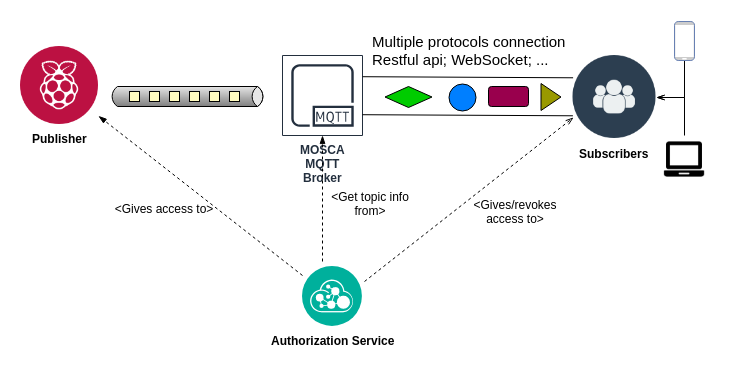
\includegraphics[width=1\textwidth]{architectureSmall.png}%
 \caption{Architecture design}
 \label{fig:architecture}
\end{center}
\end{figure}

Per i motivi sopra citati, si è reso essenziale l'implementazione di un middleware che ho chiamato authorization service (AS). Questa applicazione definisce le modalità di accesso per la pubblicazione e la fruizione dei dati che passano per il broker mqtt. Attraverso questo layer di autenticazione e autorizzazione si può dare massimo controllo dei dati al publisher che ne è il proprietario e che decide a chi dare o revocare l'accesso.

Il broker richiama l'AS per gestire l'autenticazione iniziale del cliente e l'autorizzazione del subscriber durante l'invio dei dati. In questo modo, il publisher, ha una gestione completa dei suoi dati e può decidere a quale subscriber permetterne l'accesso.

La comunicazione con il broker avviene attraverso Transport Layer Security (TLS) che permette una comunicazione sicura dalla sorgente al destinatario. Infine, per evitare che il broker possa leggere il payload del messaggio e quindi per rendere la comunicazione privata tra i due attori del sistema, ho integrato il protocollo PGP.

Il publisher quindi si registra con l'AS e comincia a pubblicare i dati su un topic. Un altro utente, che vuole diventare subscriber di quel topic, invia una richiesta al publisher per usufruire di quei dati. A questo punto il publisher può:
\begin{itemize}
    \item Rifiutare la richiesta e quindi non permettere all'utente di diventare subscriber dei suoi dai.
    \item Accettare la richiesta e aggiungere la chiave pubblica del richiedente nella catena di chiavi PGP
\end{itemize}
A questo punto un subscriber può cominciare ad usare il flusso dati provenienti dal topic selezionato.

Per implementare la piattaforma sono stati usati due framework: mosca, un broker mqtt scritto con nodejs; django rest framework, un framework python perfetto per la sua velocità di sviluppo e le tantissime librerie open source utilizzabili. Per quanto riguarda invece i db, ho selezionato Postgresql per memorizzare utenti e gestire l'autorizzazione, mentre Redis per permettere un'archiviazione persistente dei messaggi del publisher.

\newpage
\section{Broker}
Esistono vari broker mqtt, ma non molti permettono una gestione dinamica delle autorizzazioni necessaria per lo sviluppo della piattaforma. La scelta del broker da usare è ricaduta su Mosca MQTT. Mosca è un broker mqtt open source scritto in nodejs, le caratteristiche principali che lo hanno reso adatto per l'implementazione della piattaforma sono le seguenti:
\begin{itemize}
\item ampia possibilità di personalizzazione
\item MQTT 3.1 e 3.1.1 compliant
\item Implementa QoS 0 e QoS 1
\item Può essere usato facilmente all'interno di altre applicazioni nodejs.
\item Permette lo storage di pacchetti offline attraverso l'uso di qualsiasi database
\end{itemize}
\subsection{Installazione e configurazione broker Mosca}
Mosca permette una comunicazione sicura tra client e broker, attraverso protocollo TLS.

Per permettere l'autenticazione, il broker invia le credenziali dell'utente all'AS che verifica le credenziali nel db e risponde al broker permettendo o negando l'accesso.
Per permettere una comunicazione sicura tra AS e broker, quest'ultimo deve inserire nell'header delle richieste un API Key condivisa tra i due sistemi.

Un publisher può pubblicare solo su topic composti dal suo username come prima parte, in questo modo ad esempio un utente con username uguale a \textit{rossi} può pubblicare solo su topic composti da \textit{/rossi/*}.
Se è autorizzato a pubblicare, viene richiamato l'AS per salvare il nuovo topic in modo che sia visibile agli utenti che vogliono usufruire di quei dati.
Per evitare di richiamare troppo spesso l'AS, la prima risposta del server è salvata in Redis che funge anche cache del sistema.

Per quanto riguarda il subscriber, le sue richieste verso il broker sono inviate all'AS che ne verifica l'autorizzazione. Un subscriber è autorizzato quando ha inviato una richiesta al publisher e questa è stata accettata.
Anche in questo caso ho usato Redis per sfruttare la cache tra broker e AS.

Il broker definisce 4 eventi:
\begin{itemize}
    \item \emph{authenticate}. Viene richiamato quando un nuovo utente vuole cominciare ad interagire con il broker.
    \item \emph{authorizePublish}. Definisce se un publisher può pubblicare su un topic.
    \item \emph{authorizeSubscribe}. Definisce se un subscriber può \texttt{abbonarsi} ad un topic.
    \item \emph{authorizeForward}. Viene richiamato ogni volta che si deve inviare un messaggio ad un subscriber per verificare se è ancora autorizzato a riceverlo.
\end{itemize}

Un publisher può revocare l'autorizzazione ad un subscriber richiamando l'AS; in questo caso il subscriber non riceverà più i nuovi pacchetti.

\newpage
\section{Authorization Service}
L'authorization service è una RestFul API che permette la gestione degli accessi (autenticazione) e quella dei permessi (autorizzazione) oltre che tutte le azioni per accettare/revocare le richieste dei subscribers.

Per implementare l'AS ho usato Django (jang-goh).
Django è un framework utile per creare applicazioni web, è gratuito e open source ed è scritto in Python. 
Django rest framework permette di espandere le funzionalità di django per creare restful api.
Le caratteristiche principali sono:
\begin{itemize}
    \item \emph{framework modulare}. Ogni progetto di Django comprende varie app o componenti.
    \item Esistono tante componenti gratuite facilmente integrabili nel progetto e utili a sviluppare applicazioni web più velocemente.
    \item Documentazione dell'api \emph{autegenerata.}
\end{itemize}

Il database che ho scelto è Postgresql. Questo database open source è nato nell'Università della California a Berkeley. Le sue caratteristiche principali sono \cite{ionosPostgres}:
\begin{itemize}
    \item Possibilità di domande complesse
    \item Chiavi esterne (foreign keys) per il collegamento di dati da due tabelle
    \item Trigger che vengono attivati automaticamente in ingresso e controllano, confermano, modificano, eliminano o in alternativa inseriscono i dati di riferimento
    \item Visualizzazioni aggiornabili
    \item Concetto di transazione completo
    \item Multiversion Concurrency Control (MVCC) per eseguire in modo efficiente l’accesso simultaneo al database
    \item Supporta JSON
\end{itemize}

Le tabelle che ho definito sono: User, Profile, Topic, Request, API keys. 
Queste tabelle sono descritte in figura \ref{fig:database}
\begin{figure}
\begin{center}
  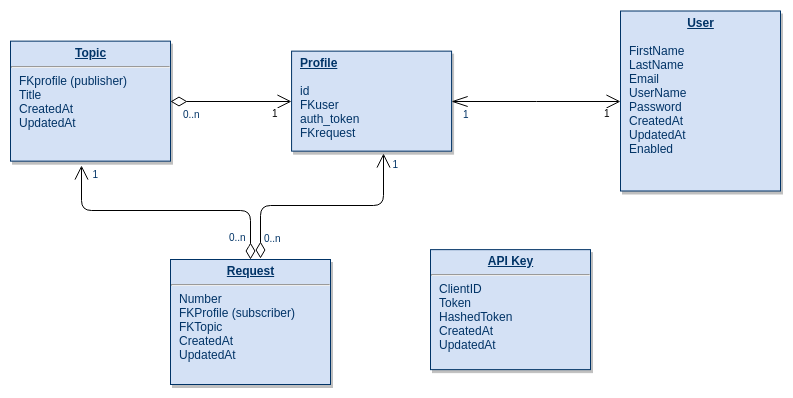
\includegraphics[width=1\textwidth]{database.png}%
  \caption{Database}
  \label{fig:database}
\end{center}
\end{figure}
Di seguito sono descritti tutti gli end-point implementati.

\subsection{Lista delle richieste}
Restituisce la lista delle richieste inviate se viene specificato role=subscriber come parametri nell'url altrimenti quelle ricevute se role=publisher.
\begin{itemize}
\item \textbf{URL} \par
    /request/
\item \textbf{Method} \par
    GET
\item \textbf{URL Params} \par
    [default: role=subscriber] role=[subscriber/publisher]
\item \textbf{Data Params} \par
    None
\item \textbf{Authorization Header} \par
    JWT <token>
\item \textbf{Success Response} \par
    \emph{Code:} 200 \par
    \emph{Content:} [requests list]
\item \textbf{Error Response} \par
    \emph{Code:} 401 UNAUTHORIZED \par
    \emph{Content:} \mint{js}|{"error": [msg] }|
    \emph{Code:} 400 BAD REQUEST \par
    \emph{Content:} \mint{js}|{"error": [msg] }|
\end{itemize}

\subsection{Invio richiesta di accesso al dato}
Crea una nuova richiesta. Inviata dal subscriber al publisher per un topic.
\begin{itemize}
\item \textbf{URL} \par
    /request/
\item \textbf{Method} \par
    POST
\item \textbf{URL Params} \par
    None
\item \textbf{Data Params} \par
    topic: <topic title>
\item \textbf{Authorization Header} \par
    JWT <token>
\item \textbf{Success Response} \par
    \emph{Code:} 200 \par
    \emph{Content:} [created request]
\item \textbf{Error Response} \par
    \emph{Code:} 401 UNAUTHORIZED \par
    \emph{Content:} \mint{js}|{"error": [msg] }|
    \emph{Code:} 400 BAD REQUEST \par
    \emph{Content:} \mint{js}|{"error": [msg] }|
\end{itemize}

\subsection{Acetta o rifiuta una richiesta}
Cambia lo stato di una richiesta per accettarla, cancellarla o rifiutarla
\begin{itemize}
\item \textbf{URL} \par
    /request/
\item \textbf{Method} \par
    PATCH
\item \textbf{URL Params} \par
    None
\item \textbf{Data Params} \par
    topic: <topic title> \par
    subscriber: <subscriber username>
\item \textbf{Authorization Header} \par
    JWT <token>
\item \textbf{Success Response} \par
    \emph{Code:} 200 \par
    \emph{Content:} [updated request]
\item \textbf{Error Response} \par
    \emph{Code:} 401 UNAUTHORIZED \par
    \emph{Content:} \mint{js}|{"error": [msg] }|
    \emph{Code:} 400 BAD REQUEST \par
    \emph{Content:} \mint{js}|{"error": [msg] }|
\end{itemize}

\subsection{Check credenziali della piattaforma}
Controlla le credenziali e ritorna un jwt token da usare in ogni 
chiamata successiva per identificare l'utente.
\begin{itemize}
\item \textbf{URL} \par
    /rest-auth/login/
\item \textbf{Method} \par
    POST
\item \textbf{URL Params} \par
    None
\item \textbf{Data Params} \par
    username; password
\item \textbf{Success Response} \par
    \emph{Code:} 200 \par
    \emph{Content:} [jwt token]
\item \textbf{Error Response} \par
    \emph{Code:} 401 UNAUTHORIZED \par
    \emph{Content:} \mint{js}|{"error": [msg] }|
    \emph{Code:} 400 BAD REQUEST \par
    \emph{Content:} \mint{js}|{"error": [msg] }|
\end{itemize}

\subsection{Lista dei topic}
Restituisce una lista di tutti i topic nel sistema.
\begin{itemize}
\item \textbf{URL} \par
    /topic/
\item \textbf{Method} \par
    GET
\item \textbf{URL Params} \par
    None
\item \textbf{Data Params} \par
    None
\item \textbf{Authorization Header} \par
    JWT <token>
\item \textbf{Success Response} \par
    \emph{Code:} 200 \par
    \emph{Content:} [topic list]
\item \textbf{Error Response} \par
    \emph{Code:} 401 UNAUTHORIZED \par
    \emph{Content:} \mint{js}|{"error": [msg] }|
\end{itemize}

\subsection{MQTT Login [Broker end-point]}
Permette l'autenticazione di un utente rispetto al broker mqtt. Questo endpoint viene richiamato dal broker quando l'utente si vuole autenticare.
\begin{itemize}
\item \textbf{URL} \par
    /login/
\item \textbf{Method} \par
    POST
\item \textbf{URL Params} \par
    None
\item \textbf{Data Params}
    username; password
\item \textbf{Success Response} \par
    \emph{Code:} 200 \par
    \emph{Content:} \mint{js}| {"token": [str]} |
\item \textbf{Error Response} \par
    \emph{Code:} 401 UNAUTHORIZED \par
    \emph{Content:} \mint{js}|{"error": [msg] }|
\end{itemize}


\subsection{Creazione di un topic [Broker end-point]}
Permette la creazione di un nuovo topic.
È il broker mqtt ad eseguire l'azione.
\begin{itemize}
\item \textbf{URL} \par
    /topic/
\item \textbf{Method} \par
    POST
\item \textbf{URL Params} \par
    None
\item \textbf{Data Params} \par
    None
\item \textbf{Header} \par
     Api-Token: YOUR\_API\_TOKEN\_HERE \par
     Api-Secret-Key: YOUR\_API\_SECRET\_KEY\_HERE
\item \textbf{Success Response} \par
    \emph{Code:} 200 \par
    \emph{Content:} [topic created]
\item \textbf{Error Response} \par
    \emph{Code:} 401 UNAUTHORIZED \par
    \emph{Content:} \mint{js}|{"error": [msg] }|
\end{itemize}

\subsection{Subscriber Authorization [Broker end-point]}
Check per verificare che un utente possa diventare un subscriber di un topic.
Verifica che lo stato della richiesta sia in Accepted
\begin{itemize}
\item \textbf{URL} \par
    /auth/
\item \textbf{Method} \par
    POST
\item \textbf{URL Params} \par
    None
\item \textbf{Header} \par
     Api-Token: YOUR\_API\_TOKEN\_HERE \par
     Api-Secret-Key: YOUR\_API\_SECRET\_KEY\_HERE
\item \textbf{Data Params} \par
    username: <subscriber username>
    topic: <topic title>
\item \textbf{Success Response} \par
    \emph{Code:} 200
    \emph{Content:} \mint{js}| {accepted request} |
\item \textbf{Error Response} \par
    \emph{Code:} 401 UNAUTHORIZED \par
    \emph{Content:} \mint{js}|{"error": [msg] }|
\end{itemize}

\subsection{Admin}
Per la gestione dell'AS viene usato l'admin panel di djagno.
Il pannello di gestione è accedibile all'url \textit{/admin/}

Oltre alla possibilità di generare/modificare/cancellare un dato nelle tabelle del db, questa applicazione serve per la creazione degli utenti e delle api Key.
\begin{figure}
\begin{center}
  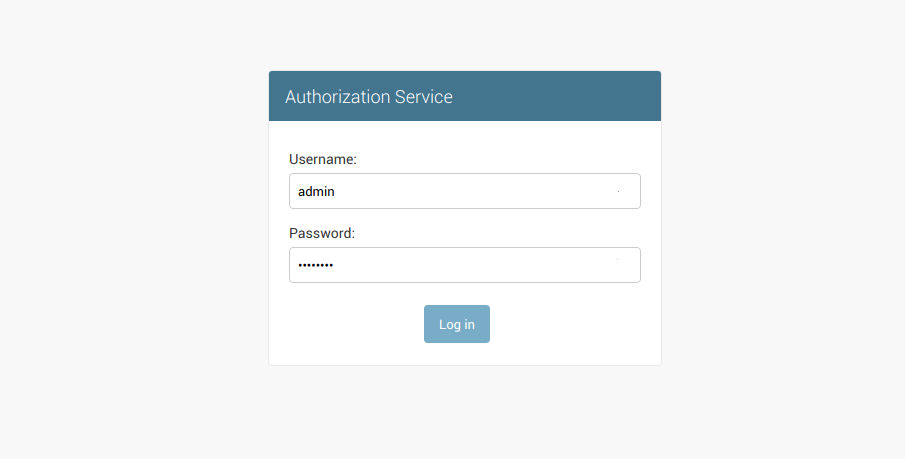
\includegraphics[width=1\textwidth]{LoginAS.png}%
  \caption{Admin login page}
  \label{fig:LoginAS}
\end{center}
\end{figure}
\begin{figure}
\begin{center}
  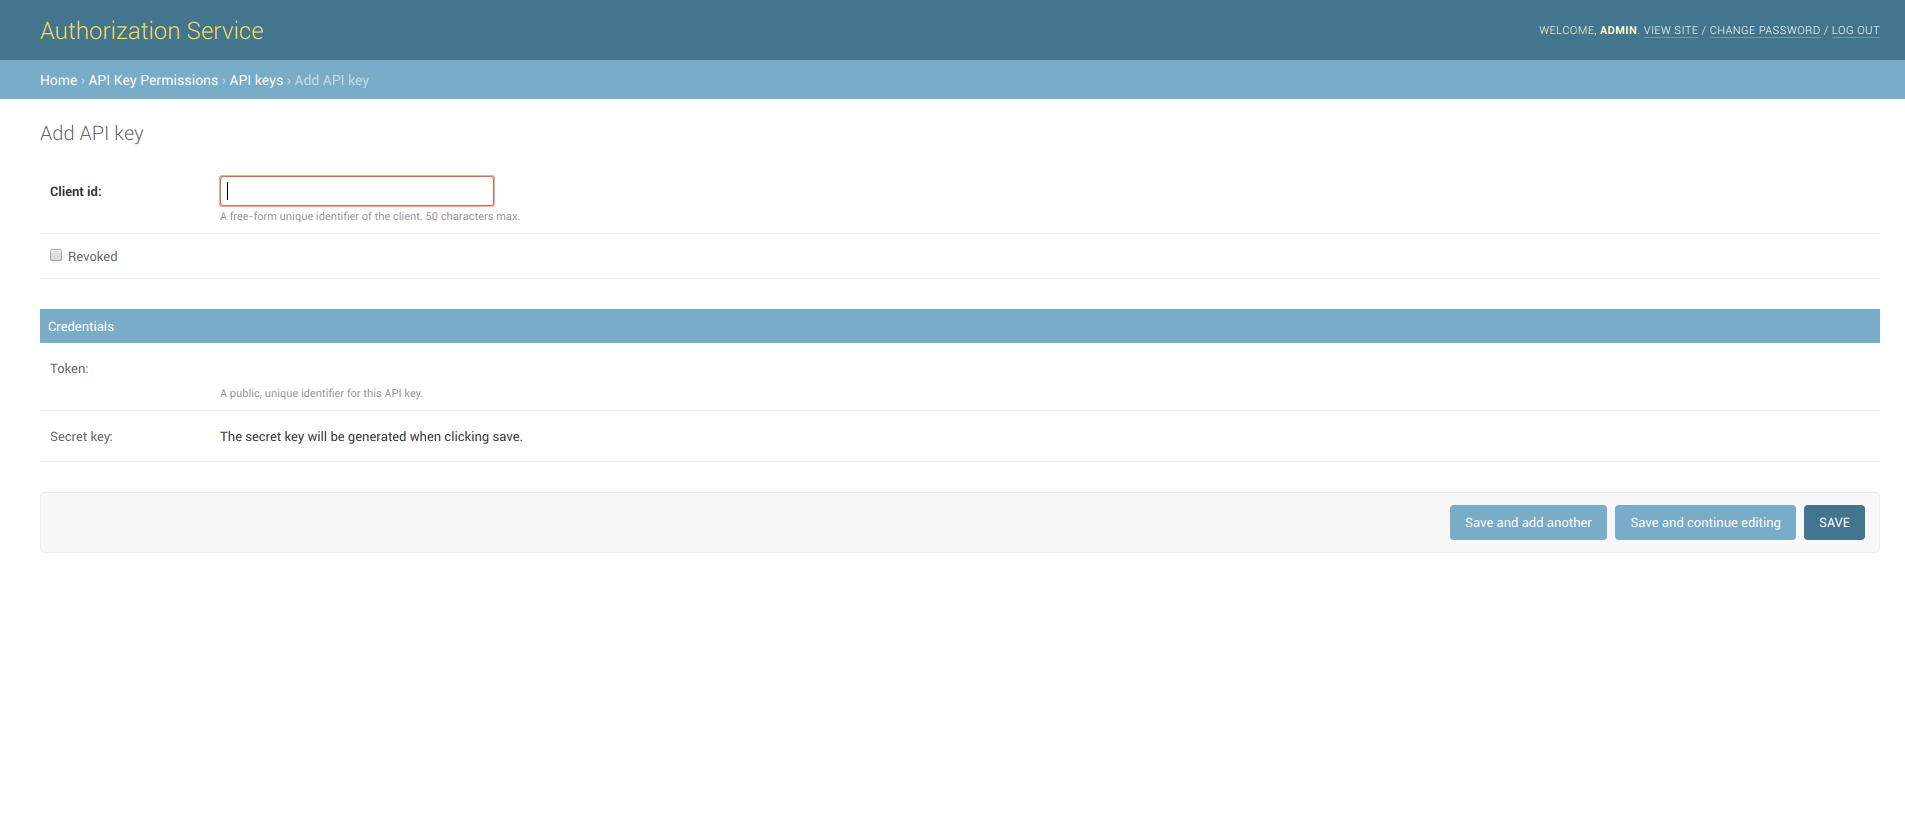
\includegraphics[width=1\textwidth]{images/AddAPIkeyAS.png}%
  \caption{Generate api key}
  \label{fig:AddAPIkeyAS}
\end{center}
\end{figure}
\begin{figure}
\begin{center}
  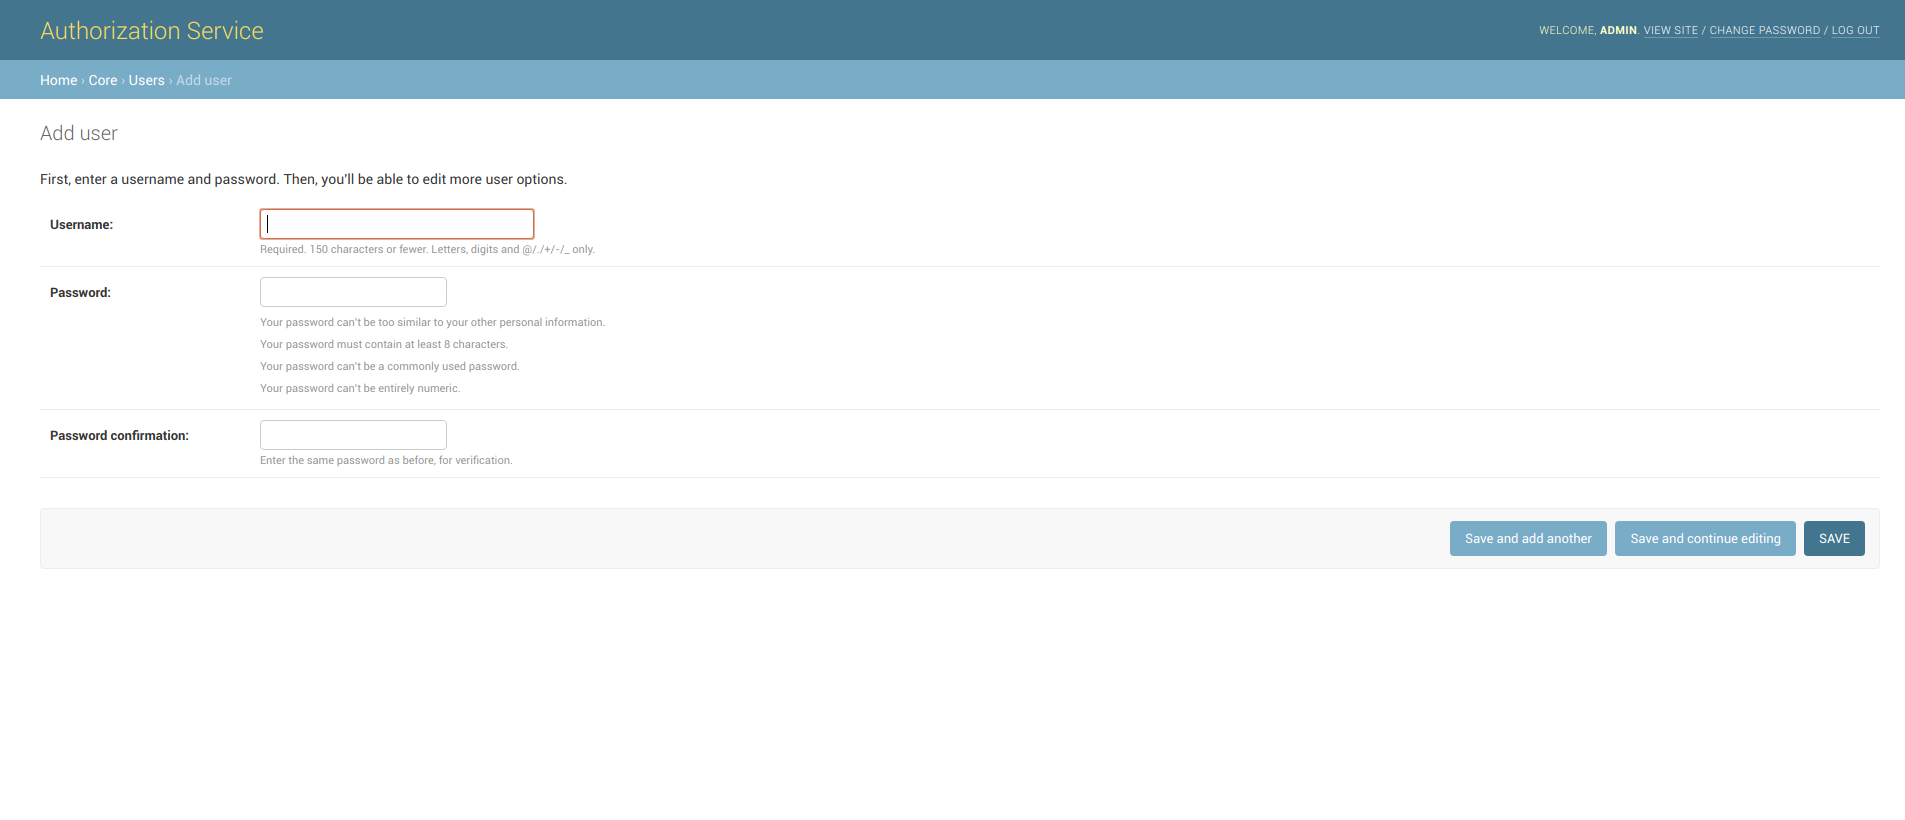
\includegraphics[width=1\textwidth]{images/AddUserAS.png}%
  \caption{Create new user}
  \label{fig:AddUserAS}
\end{center}
\end{figure}

\newpage
\section{Publisher}
Per generare il flusso di dati, ho scelto di usare un raspberry pi e un sensore per misurare il particolato che è una polvere molto fine capace di penetrare facilmente nell'apparato respiratorio.
Riguardo la dimensione delle polveri, è stata fatta una distinzione tra PM10 e PM2.5: PM10 si riferisce alle particelle più piccole di 10µm; PM2.5 sono particelle più piccole di 2.5µm. L'organizzazione Mondiale della Sanità ha fissato i limiti a:
\begin{itemize}
    \item PM10 20 µg/m³ di media l'anno
    \item PM2,5 10 µg/m³ di media l'anno
    \item PM10 50 µg/m³ di media al giorno
    \item PM2,5 25 µg/m³ di media al giorno
\end{itemize}
Nella comunità europea il limite per i PM10 è di 40 µg/m³ l'anno.

\subsection{Sensore Nova SDS011}
Per calcolare il particolato ho usato il sensore Nova SDS011 \ref{fig:sensor}.


\begin{figure}
\begin{center}
  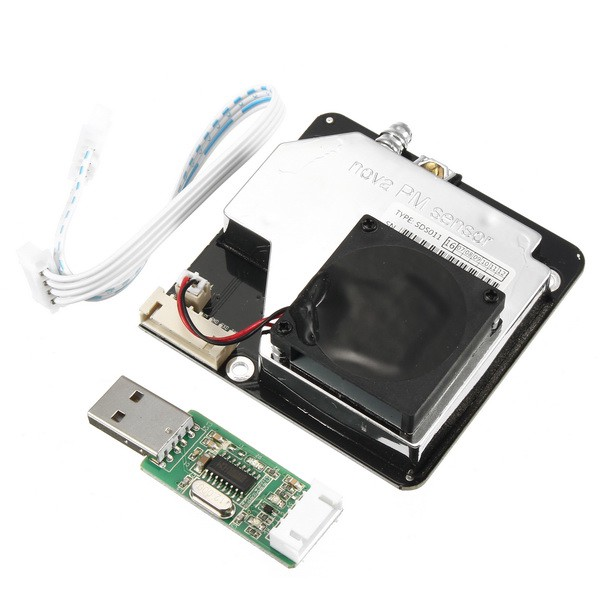
\includegraphics[width=0.6\textwidth]{particulate_sensor.jpg}%
  \caption{SDS011 sensor}
  \label{fig:sensor}
\end{center}
\end{figure}

Il sensore si collega via USB al rasberry pi. Per recuperare i dati del sensore ho usato la libreria javascript \textit{SDS011-Wrapper} \cite{pmSensorGithub}. 



\subsection{Raspberry Pi}
Il raspberry Pi è un single-board computer sviluppato nel Regno Unito dalla Raspberry Pi Foundation. Broadcom BCM2837B0, Cortex-A53 (ARMv8) 64-bit SoC @ 1.4GHz
Il modello che ho usato è un Raspberry Pi 3 model B. Il "system-on-a-chip" è di fabbricazione Broadcom (BCM2837 per Raspberry Pi 3), ed incorpora un Cortex-A53 64-bit SoC @ 1.4GHz e 1 Gigabyte di memoria. Il sistema usa una scheda SD per il boot e per la memoria non volatile.

Il raspberry non ha un sistema operativo preinstallato. Raspbian è l'os "ufficiale", è basato su Debian ed è stato creato appositamente per il raspberry dalla Raspberry Pi Foundation. 

Una volta connesso alla rete e configurato l'ssh \cite{setupraspberry}, ci si può connettere per iniziare l'implementazione del broker. 

\subsection{Implementazione}
Il flusso di creazione di un publisher è mostrato in figura \ref{fig:publisher}
\begin{figure}
\begin{center}
  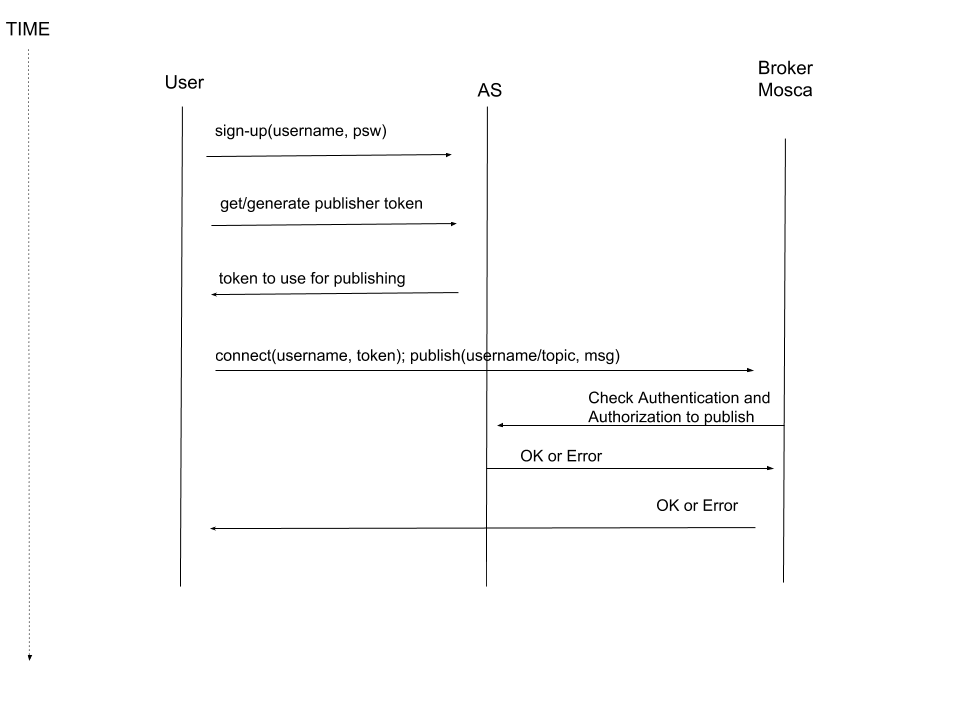
\includegraphics[width=1\textwidth]{publisher.png}%
  \caption{Flusso publisher}
  \label{fig:publisher}
\end{center}
\end{figure}

Ho usato la libreria "mqtt" di nodejs per connettere il client al broker mosca. Ogni volta che arriva una lettura dal sensore, il valore di PM10 è pubblicato sul topic selezionato (pseudo codice \ref{lst:publisher}). Poiché il tempo di vita del sensore è stimato in circa 8000 ore, è importante settare una frequenza di lettura idonea.  

\begin{lstlisting}[language=Python, caption={Publisher Pseudocode}, label={lst:publisher}]
let client = new mqtt broker connection
let topic = "username/tesi/pm10"
let sensor = new sds011 connection
sensor.on('measure', (data) => {
  client.publish(topic, data['PM10'])
});
\end{lstlisting}

Il codice completo è presentato in

\newpage
\section{Subscriber}
Un cliente che vuole diventare subscriber di un topic, deve prima richiedere l'accesso al publisher, che può dare o negare l'accesso. 

Il flusso di accesso all'informazione per un subscriber è mostrato in figura \ref{fig:subscriber}
\begin{figure}
\begin{center}
  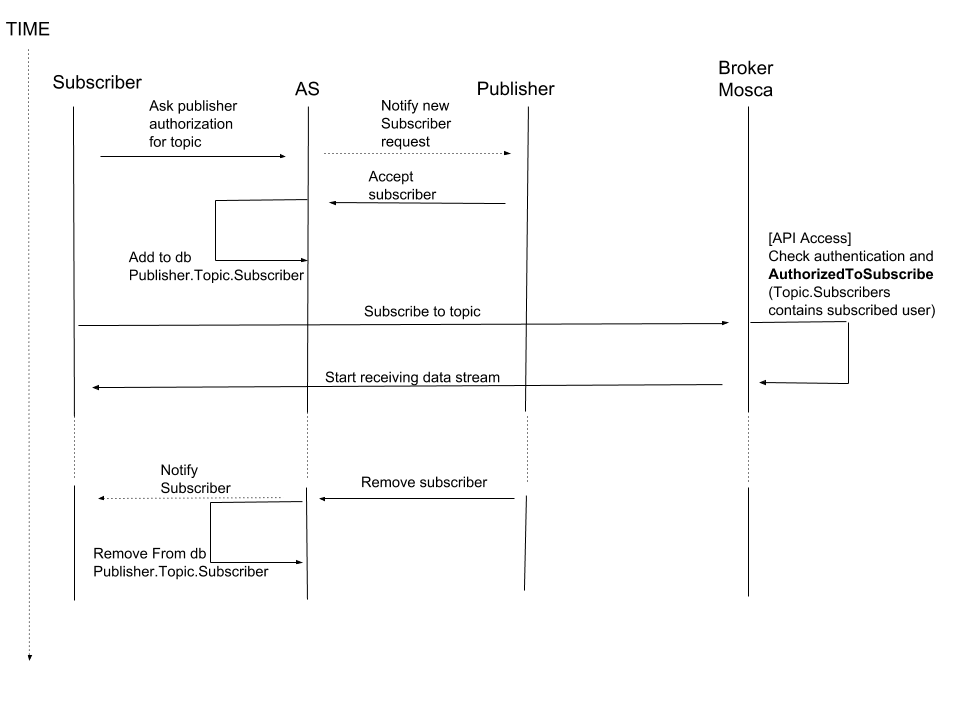
\includegraphics[width=1\textwidth]{subscriber.png}%
  \caption{Flusso subscriber}
  \label{fig:subscriber}
\end{center}
\end{figure}

Il subscriber, attraverso l'authorization service (AS), richiede al publisher l'accesso ai dati, che sempre grazie all'AS può in un primo momento concedere e in seguito revocare l'autorizzazione ai topic su cui sta pubblicando lo stream dati.

\newpage
\section{Sicurezza e E2EE}
Come ho detto all'inizio del capitolo, Mosca permette una comunicazione sicura implementando il protocollo TLS. Nonostante questa precauzione però, il messaggio è ancora visibile al server mqtt. 
Crittografia End-To-End (E2EE) vuol dire che il contenuto di un messaggio è visibile solo al mittente e al destinatario, in questo modo si evita che un intermediario, malevolo o no, possa spiare la conversazione o usare i dati di un utente in modo inappropriato.
\subsection{Pretty Good Privacy}
Il protocollo Pretty Good Privacy (PGP) è molto usato per crittografare una comunicazione one-to-one come ad esempio quella tramite mail in modo da essere sicuri che un messaggio sia letto solo dal destinatario. Esistono diverse varianti del protocollo: PGP, OpenPGP, GPG. 

Il protocollo si basa sull'uso di una coppia di chiavi pubblica/privata. La chiave pubblica è usata per crittografare un messaggio che solo con la chiave privata può essere letto.
Criptare e decriptare un messaggio su un client non è un'operazione efficiente \cite{explainPGPEncryption}.
Un'idea generale di come è implementato il protocollo è visibile in figura \ref{fig:pgp}.
\begin{figure}
\begin{center}
  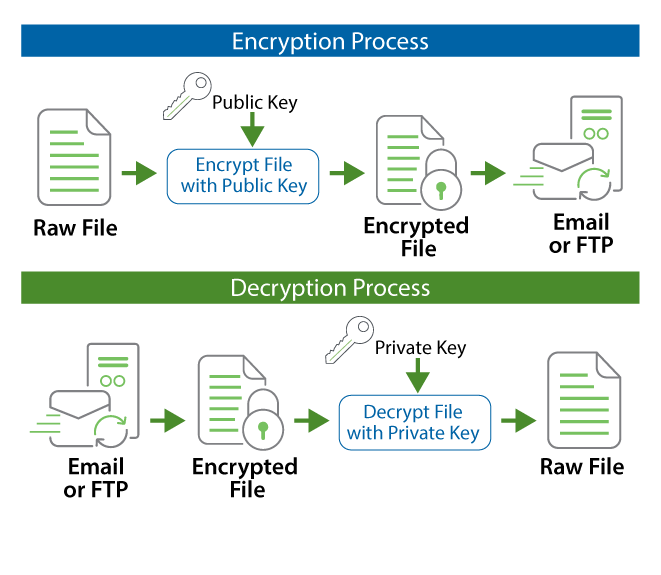
\includegraphics[width=1\textwidth]{images/OpenPGP.png}%
  \caption{PGP System \cite{OpenPGPgoanywhere}}
  \label{fig:pgp}
\end{center}
\end{figure}

PGP permette l'invio di un messaggio criptato a destinatari multipli usando tutte le chiave pubbliche dei destinatari. In questo modo, il mittente, può decidere istantaneamente di escludere un destinatario eliminando la sua chiave pubblica durante la fase di criptazione. 
\subsection{PGP e mqtt}
All'interno della piattaforma ogni cliente, durante la generazione del profilo, carica la propria chiave pubblica.
Nella richiesta per diventare un subscriber viene inserita anche la chiave pubblica dell'utente in modo che quando il publisher accetta la richiesta, questa può essere usata per crittografare il messaggio.
Quando un publisher vuole revocare l'accesso ad un subscriber, può semplicemente eliminare la chiave del subscriber in modo che quest'ultimo non possa più leggere i payloads inviati dal broker.
Il broker MQTT non può leggere i messaggi scambiati all'interno del sistema e si limita alla gestione dei flussi.


\section{Pregi, limiti e prospettive future}
Testo sezione
non è implementato in modo chiaro come avere la lista dei topic
La security è opzionale

